% Generated by experiments/plot_ch3_parametric.py. Preamble: \usepackage{graphicx}
\begin{figure}[htbp]
  \centering
  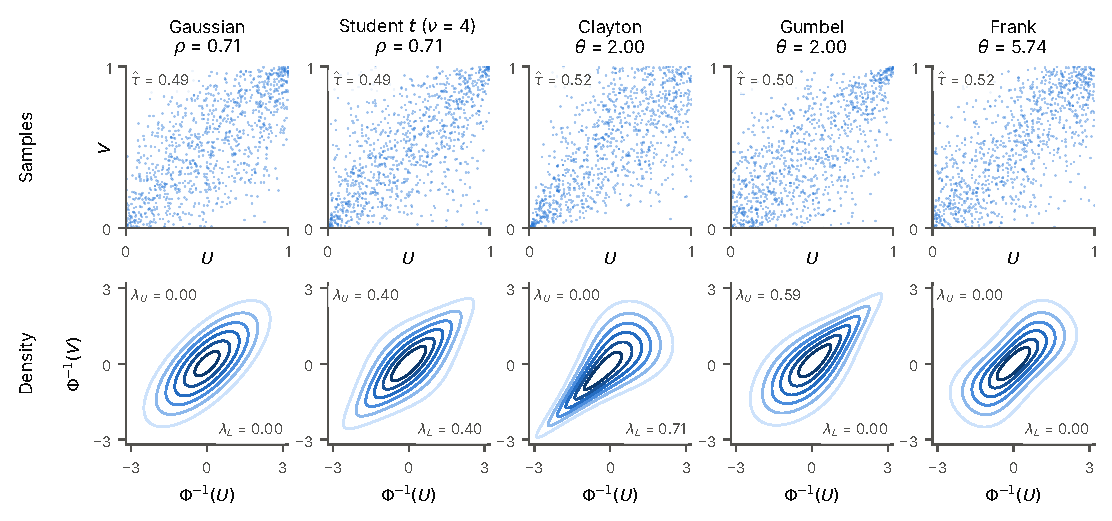
\includegraphics[width=\textwidth]{figures/fig_ch3_parametric}
  \caption{The five copula families of Table~\ref{tab:copula-families}, each with its
    parameter chosen so that Kendall's $\tau = 0.5$. Top: $n = 1000$ samples on the copula
    scale $(U,V)$, with the sample $\hat\tau$. Bottom: the copula density on normal scores
    $\bigl(\Phi^{-1}(U),\Phi^{-1}(V)\bigr)$, contours at $0.01, 0.03, 0.06, 0.10, 0.15$ and
    $0.20$ in every panel, with the lower and upper tail-dependence coefficients $\lambda_L$
    and $\lambda_U$. Equal $\tau$ does not fix the tails: Clayton concentrates dependence in
    the lower tail, Gumbel in the upper tail, the Student~$t$ in both, and the Gaussian and
    Frank copulas in neither.}
  \label{fig:ch3-parametric}
\end{figure}
